% !TEX root = flow_head.tex
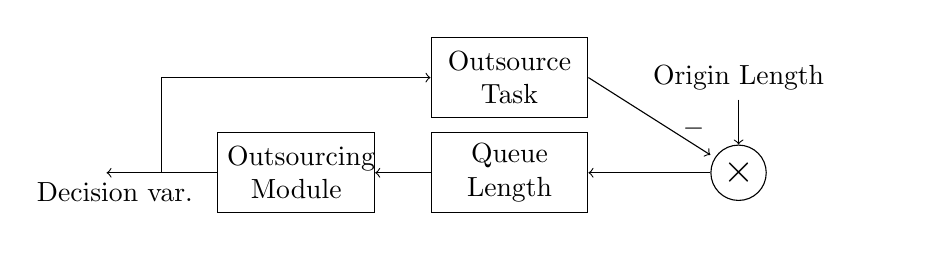
\begin{tikzpicture}[node distance=5mm and 5mm,
square/.style={
% The shape:
rectangle,
draw=black,
minimum size=2.9em,
text width=5em,
text centered
},
coord/.style={
coordinate,
% on chain,
% on grid,
% node distance=6mm and 25mm
},
circle/.style={
rectangle,minimum size=2em,rounded corners=1em,
draw=black
},
skip loop/.style={to path={-- ++(0,#1) -| (\tikztotarget)}}
]
\matrix[row sep=0.5em,column sep=2em] {
% First row:
& & &   \node	(out) [square] {Outsource Task} ; &  \node (originl) {Origin Length} ; & \\
\node (end1) [coord] {}; & \node (node1) [coord] {} ; & \node (outsource) [square] {Outsourcing Module} ; &\node (length) [square] {Queue Length} ; & \node (compare1) [circle] {\Large$\times$};  & \\
&  & &  & &\\
};
\path (originl) edge[->] (compare1) (compare1) edge[->] (length) (length) edge[->] (outsource) (outsource) edge[->] (end1);
\path (out.east) edge[->] (compare1);
\draw [->] (node1) |- (out) ;
\path (out) to node [near end,xshift=0.5em,yshift=0.7em] {$-$} (compare1) (outsource) to node [near end,yshift=-0.7em,xshift = -0.7em] {Decision var.} (end1);
\end{tikzpicture}